% 需要 amsmath、amssymb、graphicx；配图仅使用PDF。
\subsubsection{基于MediaPipe的视觉特征提取}

视觉支路侧重提取面部变化线索。眉部运动、眼睑开合和嘴部形态等变化能够补充文本语义与发声方式，因此本文采用MediaPipe Face Landmarker输出的面部blendshape系数作为视觉表示。该表示具有固定的维度与字段名称，便于逐帧记录并按时间聚合，其描述范围主要是面部形态与表情变化，不覆盖画面中的全部场景信息或肢体动作。按输出字段分组，52维系数的组成及代表性含义见表~\ref{tab:p1_visual_groups}。

\begin{table}[htbp]
    \centering
    \caption{52维面部系数的分组及代表性含义}
    \label{tab:p1_visual_groups}
    \begingroup
    \small
    \renewcommand{\arraystretch}{1.2}
    \begin{tabular}{@{}p{0.14\linewidth}p{0.43\linewidth}p{0.25\linewidth}r@{}}
        \hline
        分组 & 代表性输出 & 主要描述内容 & 维度\\ \hline
        额眉部 & 压眉、内侧抬眉、外侧抬眉 & 眉部位置与形态 & 5\\
        眼部 & 眨眼、睁大、眯眼及视线方向 & 眼睑状态与眼部运动 & 14\\
        面颊与鼻部 & 鼓腮、面颊收紧、鼻部牵动 & 面中部形态 & 5\\
        嘴部 & 嘴角上扬或下压、噘嘴、嘴唇收紧等 & 嘴唇及嘴角形态 & 23\\
        下颌 & 张嘴、下颌前伸及左右移动 & 下颌位置与开合 & 4\\
        其他输出项 & 工具字段\texttt{\_neutral} & 保留输出，不作为中性情感判据 & 1\\ \hline
        合计 & & & 52\\ \hline
    \end{tabular}
    \endgroup
\end{table}

该方法包含人脸检测、面部关键点估计与表情系数预测三个环节。首先定位画面中的人脸区域，再估计面部关键点，最后由预训练模型将关键点信息映射为52维系数。设第$m$个抽样画面为$I_m$，选定人脸的关键点集合为$P_m$，则这一过程可概括为
\begin{equation}
    P_m=f_{\mathrm{landmark}}(I_m),\qquad
    \boldsymbol{c}_m=g_{\mathrm{blendshape}}(P_m)
    \in\mathbb{R}^{52},
    \label{eq:p1_visual_mapping}
\end{equation}
其中$f_{\mathrm{landmark}}$概括人脸检测、关键点估计及目标人脸选择，$g_{\mathrm{blendshape}}$表示预训练的表情系数映射。本文使用已有模型参数，不利用本问的情感标签进行微调。各分量描述不同面部形态的激活程度，多个分量可以同时较高，不构成相互排斥的情感类别概率分布。

本文保留各系数的连续输出，而不将其转换为单一表情类别，以记录多个面部部位的共同变化及其随时间的变化幅度。对于具有左右侧区分的分量，分别保留对应输出，以记录可能存在的面部运动不对称性。所有帧均采用相同的字段顺序，使同一列始终对应同一种面部描述量，为后续按词区间聚合提供一致的特征含义。

对预处理得到的抽样帧逐帧进行检测，不在帧间额外引入跟踪或平滑。当同一画面检测到多张人脸时，根据关键点包围区域的面积选择最大人脸作为当前帧的特征来源。这是一项统一的选择规则，并不保证所选人脸一定属于说话者。对于没有获得可用面部特征的画面，保留该帧位置，以零向量占位并设置无效标记，避免将观测缺失解释为中性表情。设视觉观测有效标记为$o_m^{(V)}\in\{0,1\}$，保存的视觉特征为
\begin{equation}
    \boldsymbol{v}_m=
    \begin{cases}
        \boldsymbol{c}_m, & o_m^{(V)}=1,\\
        \boldsymbol{0}, & o_m^{(V)}=0.
    \end{cases}
    \label{eq:p1_visual_observation}
\end{equation}
有效帧中某个系数较低，表示该分量的模型输出较低；无效帧中的全零向量仅用于占位，不能作为实际面部观测参与聚合。

为展示系数变化与观测缺失的区别，选取样本\texttt{-wny0OAz3g8\$\_\$9}，将实际抽样画面、张嘴系数、左右嘴角上扬系数和左右眼睑闭合系数置于同一时间记录下，如图~\ref{fig:p1_visual_example}所示。该样本共包含31个抽样帧，其中29帧获得可用面部特征。图中曲线直接读取已有输出，缺失位置以断线表示；底部标记显示各抽样时刻的观测有效性。该样本用于说明特征含义与缺失处理，不代表全体样本的检测表现。

\begin{figure}[htbp]
    \centering
    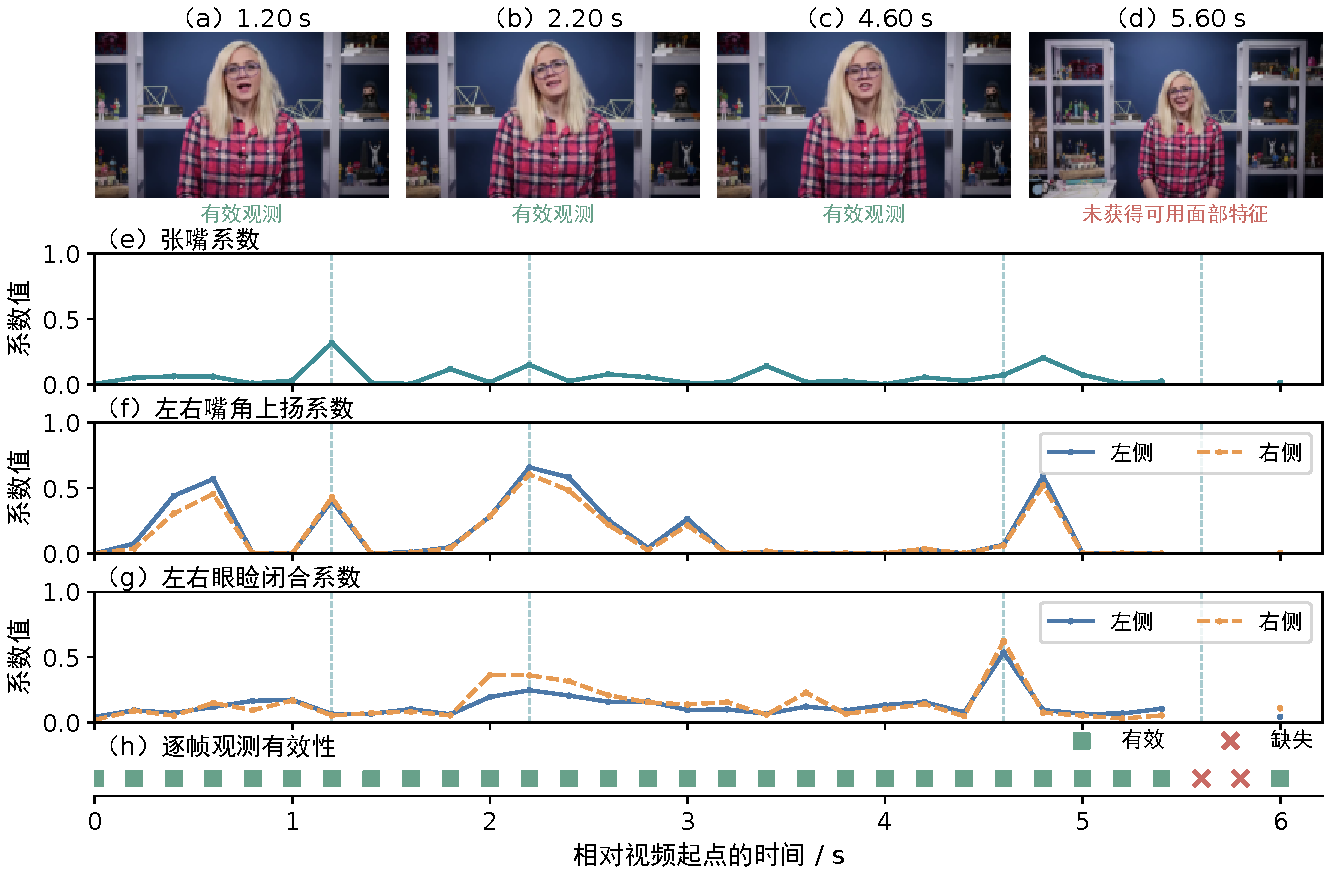
\includegraphics[width=\textwidth]{figures/fig_5_3_visual_example.pdf}
    \caption{同一视频片段的实际画面、代表性面部系数与观测有效性。竖向虚线标示上方四帧的实际时刻；曲线上的点对应抽样帧，连线仅辅助观察变化，无效位置不连接。}
    \label{fig:p1_visual_example}
\end{figure}

在1.20 s处，张嘴系数为0.318，对应画面中可见的张口形态；在2.20 s处，左右嘴角上扬系数分别为0.659和0.605；在4.60 s处，左右眼睑闭合系数分别升至0.535和0.623。不同系数在不同位置呈现变化，说明保留多维连续表示能够分别记录各面部部位的运动线索。这些数值描述模型对面部形态的输出，不能直接解释为某种情感的概率。

在5.60 s和5.80 s处，工具未获得可用面部特征，因而对应位置的观测标记为0。图中5.60 s的画面仍可见人物，表明“未获得可用面部特征”不能直接等同于“画面无人”。这两帧的占位零向量不作为表情变化绘入曲线，也不参与后续有效特征的加权聚合。

按抽样顺序排列后，得到原生视觉特征矩阵$V\in\mathbb{R}^{N_v\times52}$，其中$N_v$为抽样帧数。每行特征另关联实际时间戳$t_m^{(V)}$、原视频帧索引和观测有效标记，使各行能够回溯至具体画面。时间及有效标记均不计入52维特征，后续聚合时与特征矩阵共同使用。

综合三条特征提取支路，每条视频形成词级文本表示、窗口级声学表示和帧级视觉表示：
\begin{equation}
    X^{(T)}\in\mathbb{R}^{L\times768},\qquad
    A\in\mathbb{R}^{N_a\times25},\qquad
    V\in\mathbb{R}^{N_v\times52}.
    \label{eq:p1_native_features}
\end{equation}
其中$L$、$N_a$和$N_v$分别为词数、声学记录数和抽样视频帧数。三个矩阵的行具有不同的组织单位，尚不能直接按序列位置对应。下一节将结合给定转写与音频估计词级时间边界，再依据时间交叠关系聚合有效声学与视觉特征，建立统一词位置的三模态表示。
